
\documentclass[tikz,border=8pt]{standalone}
\usepackage{amsmath}
\usetikzlibrary{arrows.meta, positioning, calc, fit, backgrounds}

\definecolor{forward}{HTML}{2AA198}
\definecolor{backward}{HTML}{D95F5F}
\definecolor{nodeblue}{HTML}{3A86B7}
\definecolor{nodeorange}{HTML}{F28E2B}
\definecolor{lightgray}{HTML}{D9D9D9}

\begin{document}
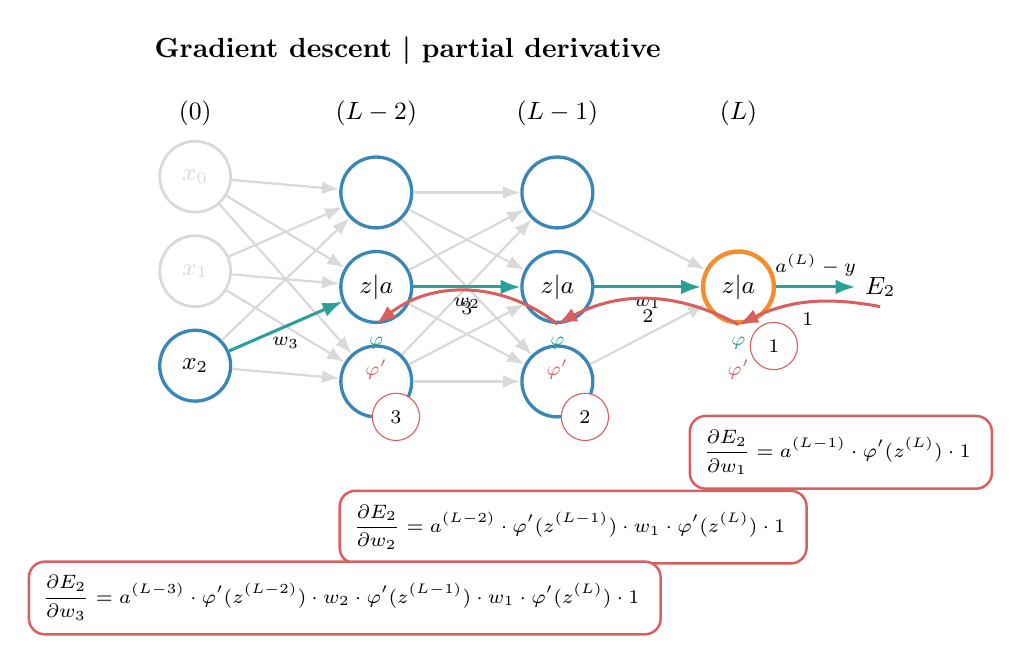
\begin{tikzpicture}[
    neuron/.style={
        circle,
        draw=nodeblue,
        line width=1.2pt,
        minimum size=9mm,
        inner sep=1pt,
        fill=white,
        font=\small
    },
    active/.style={
        circle,
        draw=nodeorange,
        line width=1.6pt,
        minimum size=9mm,
        inner sep=1pt,
        fill=white,
        font=\small
    },
    faded/.style={
        circle,
        draw=lightgray,
        line width=1pt,
        minimum size=9mm,
        inner sep=1pt,
        fill=white,
        text=lightgray,
        font=\small
    },
    arrowf/.style={
        -{Latex[length=2.5mm]},
        line width=1.1pt,
        draw=forward
    },
    arrowb/.style={
        -{Latex[length=2.5mm]},
        line width=1.1pt,
        draw=backward
    },
    grayarrow/.style={
        -{Latex[length=2.2mm]},
        line width=.8pt,
        draw=lightgray
    },
    eqbox/.style={
        rounded corners=2mm,
        draw=backward,
        line width=.9pt,
        fill=white,
        align=left,
        inner sep=5pt,
        font=\scriptsize
    }
]

% ------------------------------------------------
% Layer coordinates
% ------------------------------------------------
\node[faded]  (x0) at (0,  1.4) {$x_0$};
\node[faded]  (x1) at (0,  0.2) {$x_1$};
\node[neuron] (x2) at (0, -1.0) {$x_2$};

\node[neuron] (h1a) at (2.3,  1.2) {};
\node[neuron] (h1b) at (2.3,  0.0) {$z|a$};
\node[neuron] (h1c) at (2.3, -1.2) {};

\node[neuron] (h2a) at (4.6,  1.2) {};
\node[neuron] (h2b) at (4.6,  0.0) {$z|a$};
\node[neuron] (h2c) at (4.6, -1.2) {};

\node[active] (out) at (6.9, 0) {$z|a$};

\node[font=\small] at (0,   2.2) {$(0)$};
\node[font=\small] at (2.3, 2.2) {$(L-2)$};
\node[font=\small] at (4.6, 2.2) {$(L-1)$};
\node[font=\small] at (6.9, 2.2) {$(L)$};

% ------------------------------------------------
% Faded dense connections
% ------------------------------------------------
\foreach \i in {x0,x1,x2}{
  \foreach \j in {h1a,h1b,h1c}{
    \draw[grayarrow] (\i) -- (\j);
  }
}

\foreach \i in {h1a,h1b,h1c}{
  \foreach \j in {h2a,h2b,h2c}{
    \draw[grayarrow] (\i) -- (\j);
  }
}

\foreach \i in {h2a,h2b,h2c}{
  \draw[grayarrow] (\i) -- (out);
}

% ------------------------------------------------
% Highlighted forward path
% ------------------------------------------------
\draw[arrowf] (x2) -- node[below, font=\scriptsize] {$w_3$} (h1b);
\draw[arrowf] (h1b) -- node[below, font=\scriptsize] {$w_2$} (h2b);
\draw[arrowf] (h2b) -- node[below, font=\scriptsize] {$w_1$} (out);

\node[font=\scriptsize, text=forward] at (2.3,-.72) {$\varphi$};
\node[font=\scriptsize, text=forward] at (4.6,-.72) {$\varphi$};
\node[font=\scriptsize, text=forward] at (6.9,-.72) {$\varphi$};

% ------------------------------------------------
% Output error
% ------------------------------------------------
\node[font=\small] (err) at (8.7, 0) {$E_2$};
\draw[arrowf] (out) -- node[above, font=\scriptsize] {$a^{(L)}-y$} (err);

% ------------------------------------------------
% Backpropagation arrows
% ------------------------------------------------
\draw[arrowb, bend right=18] (err.south) to node[below, font=\scriptsize] {$1$} (out.south);
\draw[arrowb, bend right=28] (out.south) to node[below, font=\scriptsize] {$2$} (h2b.south);
\draw[arrowb, bend right=38] (h2b.south) to node[below, font=\scriptsize] {$3$} (h1b.south);

\node[font=\scriptsize, text=backward] at (6.9,-1.05) {$\varphi'$};
\node[font=\scriptsize, text=backward] at (4.6,-1.05) {$\varphi'$};
\node[font=\scriptsize, text=backward] at (2.3,-1.05) {$\varphi'$};

% ------------------------------------------------
% Number markers
% ------------------------------------------------
\node[circle, draw=backward, fill=white, minimum size=6mm, font=\scriptsize] at (7.35,-.75) {1};
\node[circle, draw=backward, fill=white, minimum size=6mm, font=\scriptsize] at (4.95,-1.65) {2};
\node[circle, draw=backward, fill=white, minimum size=6mm, font=\scriptsize] at (2.55,-1.65) {3};

% ------------------------------------------------
% Equation callout boxes
% ------------------------------------------------
\node[eqbox] (eq1) at (8.2,-2.1) {
$ \displaystyle
\frac{\partial E_2}{\partial w_1}
=
a^{(L-1)} \cdot \varphi'(z^{(L)}) \cdot 1
$
};

\node[eqbox] (eq2) at (4.8,-3.05) {
$ \displaystyle
\frac{\partial E_2}{\partial w_2}
=
a^{(L-2)} \cdot \varphi'(z^{(L-1)})
\cdot w_1 \cdot \varphi'(z^{(L)}) \cdot 1
$
};

\node[eqbox] (eq3) at (1.9,-3.95) {
$ \displaystyle
\frac{\partial E_2}{\partial w_3}
=
a^{(L-3)} \cdot \varphi'(z^{(L-2)})
\cdot w_2 \cdot \varphi'(z^{(L-1)})
\cdot w_1 \cdot \varphi'(z^{(L)}) \cdot 1
$
};

% ------------------------------------------------
% Title
% ------------------------------------------------
\node[font=\bfseries] at (2.7, 3.0) {Gradient descent \textbar{} partial derivative};

\end{tikzpicture}
\end{document}
